\documentclass{beamer}
% use this instead for 16:9 aspect ratio:
%\documentclass[aspectratio=169]{beamer}
\usepackage{etex}
\usepackage{graphicx}
\usepackage[framemethod=default]{mdframed}
\usepackage{lipsum}
\usepackage{color}
\usepackage[normalem]{ulem}
\usepackage{multicol}
\usepackage{multirow}
\usepackage{verbatim}
\usepackage{adjustbox}
\usepackage{comment}
\usepackage{cite}
\usepackage{amsmath}
\usepackage{amssymb}
\usepackage{amstext}


\newcommand{\pa}{\partial}
\newcommand{\ms}{\mathscr}
\newcommand{\xx}{{\bf x}}
\newcommand{\xd}{{\bf x}^{\dagger}}
\newcommand{\ttt}{{\ms T}}
\newcommand{\td}{{\ms T^{\dagger}}}
\newcommand{\la}{\langle}
\newcommand{\ra}{\rangle}
\newcommand{\beq}{\begin{equation}}
\newcommand{\eeq}{\end{equation}}
\newcommand{\mL}{{\ms L}}

\setbeamerfont{footnote}{size=\tiny}

\reserveinserts{28}
\usetheme{ETHbeamer}

\colorlet{ETHcolor1}{ETHc}
\colorlet{ETHcolor2}{ETHi}

\author{Guangyu Li, Jiawen Luo, Zhichao Han}

\title{Optimal resources distribution to disaster spreading}

% \date{2016-10-24}
\date{}
\usefonttheme{professionalfonts}
% uncomment if you do not want to use a department logo
%\deplogofalse

\begin{document}
\setbeamertemplate{caption}{\raggedright\insertcaption\par}
\titleframe



\section{introduction}
\begin{frame}
	\frametitle{Optimal resources distribution to disaster spreading}
	Our presentation is organized as follows:

	\begin{itemize}
		\setlength\itemsep{1em}
		\item Background: disaster spreading model and research question
		\item Methods: how to find optimal strategy to distribute resources
		\begin{itemize}
			\item PDE-constrained optimization \& Adjoint method
		\end{itemize}

		\item Results: comparison of different strategies
	\end{itemize}
\end{frame}

\begin{frame}
\begin{center}
	\Huge Background
\end{center}
\end{frame}

\begin{frame}
	\frametitle{Disaster spreading model}
	Based on original paper\footnotemark[1]
	\footnotetext[1]{L Buzna, K Peters, H Ammoser, C K\"uhnert, D Helbing, PRE 75 (5), 056107}, the disaster spreading could be modeled as:
	\begin{itemize}
		\item the system containing interacted unities $\Rightarrow$ $G=(V, E)$
		\item unit $i$ has influence to unit $j$ $\Rightarrow$ a link from node $i$ to node $j$
		\item state of node $i$ at time $t$: $x_i(t) \in \mathbb{R}^{+}$
		\item $0\leq x_i< \theta_i$: node $i$ is not failed; $\theta_i \leq x_i$: node $i$ is failed
	\end{itemize}
	The dynamic of node $i$ is modeled by formula (\ref{eq:dynamic}):
	\begin{equation}
		\label{eq:dynamic}
		\frac{dx_i}{dt} = - \frac{x_i}{\tau_i} + \Theta_i ( \sum_{i\neq j}\frac{M_{ji}x_j(t-t_{ji})}{f(O_j)} e^{-\beta t_{ji}} )
	\end{equation}
	%
	% where $\tau_i$ is the funtion of external resources on node $i$
\end{frame}

\begin{frame}
	\frametitle{Research question}
	In original paper\footnotemark[1]
	\footnotetext[1]{L Buzna, K Peters, H Ammoser, C K\"uhnert, D Helbing, PRE 75 (5), 056107}, the author compared six heuristic strategies to distribute resources.

	However there exist lots of other heuristic strategies since the ways to distribute resources are infinite.
	\pause

	\vspace{4mm}
	\Large\textbf{what is the optimal strategy?}
	% \begin{itemize}
	% 	\item In original paper\footnote{L Buzna, K Peters, H Ammoser, C K\"uhnert, D Helbing, PRE 75 (5), 056107}, the author compared six heuristic strategies to distribute resources
	% 	\item however there exist lots of other heuristic strategies since the ways to distribute resources are infinite
	% \end{itemize}
\end{frame}

\section{Adjoint Method}
\begin{frame}
\begin{center}
	\Huge {Methods}
\end{center}
\end{frame}

\begin{frame}{Resource distribution as optimization problem}
	\begin{block}{}
		We find this problem could be modeled as an optimization problem: 
	\end{block}
	\begin{itemize}
		\item Objective function:
		\begin{itemize}
			\item $J = \sum_i \Phi_i(x_i) $ minimizes the number of damaged nodes at end time $t = T$
			\item $J = \sum_i x_i $ minimizes the averaging status of all nodes
		\end{itemize}
		\item Constraints: 
			\begin{itemize}
				\item  $\frac{\pa {\xx}}{\pa t} - (K-P)\xx = 0 $ 
				\item  $\sum_i^N R_i(t) = R(t)$
			\end{itemize}
	\end{itemize}
\end{frame}

\begin{frame}{Forward Equation}
	\begin{block}{}
		\begin{center}
			 $\frac{\pa {\xx}}{\pa t} = (K-P)\xx  $ 
		\end{center}
		in which $P(t)$ is a diagonal matrix
		\begin{center}
			$P_{ij}(k) = \frac 1 {\tau_i(k)} \delta_{ij} = \frac{1}{(\tau_{start} - \beta_2)e^{-\alpha_2\sum_{t = 1}^{k}\Delta R_i(t)} + \beta_2}\delta_{ij}$
		\end{center}
	and $K$ is also a matrix with each element of $K$ as an integration kernel,
	\begin{center}
		$K_{ij}(t, s) = \frac{M_{ji}e^{-\beta t_{ji}}}{f(O_j)} \delta(s-t+t_{ji})$
	\end{center}
	\end{block}
\end{frame}

\begin{frame}{The Lagrangian}
	Formulate the Lagrangian as:
	$\begin{aligned}
		L = & \sum_{i} f(x^{(i)}_T) + \int_{0}^{T} \la\tilde{\xd}, \frac{\pa \tilde{\xx}}{\pa t} - (K - P)\tilde{\xx}\ra dt \\
		+  &\int_{10}^{T} \la\tilde{\xd_l}, \frac{\pa \tilde{\xd_l}}{\pa t} - (K - P)\tilde{\xd_l}\ra dt + \sum_{t=1}^{Nt}\lambda_t(\sum_{i}\Delta R_i(t) - \Delta R(t))
	 \end{aligned}$
	
\end{frame}

\begin{frame}{Take variations of the Lagrangian}
	\begin{itemize}
		\item Adjoint equation: 
		
			$\small \begin{aligned}
				& -\frac{\pa x_i^\dagger}{\pa t} = \sum_{j}(K^\dagger_{ij} - P(t)_{ij})x_j^\dagger, \forall i\not=l, t\in[0, T] \\
				& -\frac{\pa x_l^\dagger}{\pa t} = \sum_{j}(K^\dagger_{lj} - P(t)_{lj})x_j^\dagger, t\in[10, T]
			\end{aligned}$
		\item Compatibility condition: $(x^\dagger_T)^{(i)} = -f'(x_T^{(i)})$
		\item Gradient:
		
			{\small$\begin{aligned}
			&\frac{\pa L}{\pa \Delta R_i(t)} = \lambda_t + \int_{0}^{T} \la\frac{\pa P}{\pa \Delta R_i(t)}\tilde{\xx}, \tilde{\xd}\ra dt + \int_{10}^{T} \la\frac{\pa P}{\pa \Delta R_i(t)}\tilde{\xx}_l, \tilde{\xd}_l\ra dt \\
			&= \lambda_t + \sum_{j=t}^{T} w_j\Delta t[\frac{\pa P_{ii}(j)}{\pa \Delta R_i(t)}]x_i(j)x_i^\dagger(j) + \sum_{j=\max(t, 10)}^{T} w_j\Delta t[\frac{\pa P_{ll}(j)}{\pa \Delta R_l(t)}]x_l(j)x_l^\dagger(j).
			\end{aligned}$}
	\end{itemize}
\end{frame}

\begin{frame}{Algorithm}
	\begin{itemize}
		\item Start from random strategy or an existed one
		\item Do {\color{red}once forward simulation} $\rightarrow \xx$
		\item Calculate $\xd_T$ from compatibility condition
		\item Do {\color{red}once backward simulation} $\rightarrow \xd$
		\item Compute $\lambda_t$ from constraint: $\sum_{i}\Delta R_i(t) - \Delta R(t) = 0$
		\item Calculate $\frac{\pa L}{\pa \Delta R_i(t)}$.
		\item Update strategy as $\Delta R_i(t) \leftarrow \Delta R_i(t) - \Delta\cdot\frac{\pa L}{\pa \Delta R_i(t)}$
		\item Normalization: $\Delta R_i(t) \longmapsto \frac {\mathbb{I}_{x>0}(\Delta R_i(t))} {\|\Delta R_i(t)\|} \Delta R(t)$
		\item Return to second step if not yet converged
		
	\end{itemize}
\end{frame}


\section{Results}
\begin{frame}
\begin{center}
	\Huge Results
\end{center}
\end{frame}

% \begin{frame}
% 	\frametitle{Experiment Settings}
% \end{frame}

\begin{frame}
	\frametitle{Minimize the number of damaged nodes}
	0-1 loss funtion:
	\begin{equation}
		\label{eq:0_1_loss}
		% \begin{aligned}
			J = \sum_i h(x_i) \quad\quad
			\text{where } h(\cdot) = 
			\begin{cases}
				1 & \text{if } x_i \ge \theta_i \\
				0 & \text{otherwise}
			\end{cases}
		% \end{aligned}
	\end{equation}

	But, it is \textbf{not differentiable!}\\

	% \vspace{2mm}

	\begin{columns}
		\begin{column}{0.5\textwidth}
			\begin{figure}
			\centering
			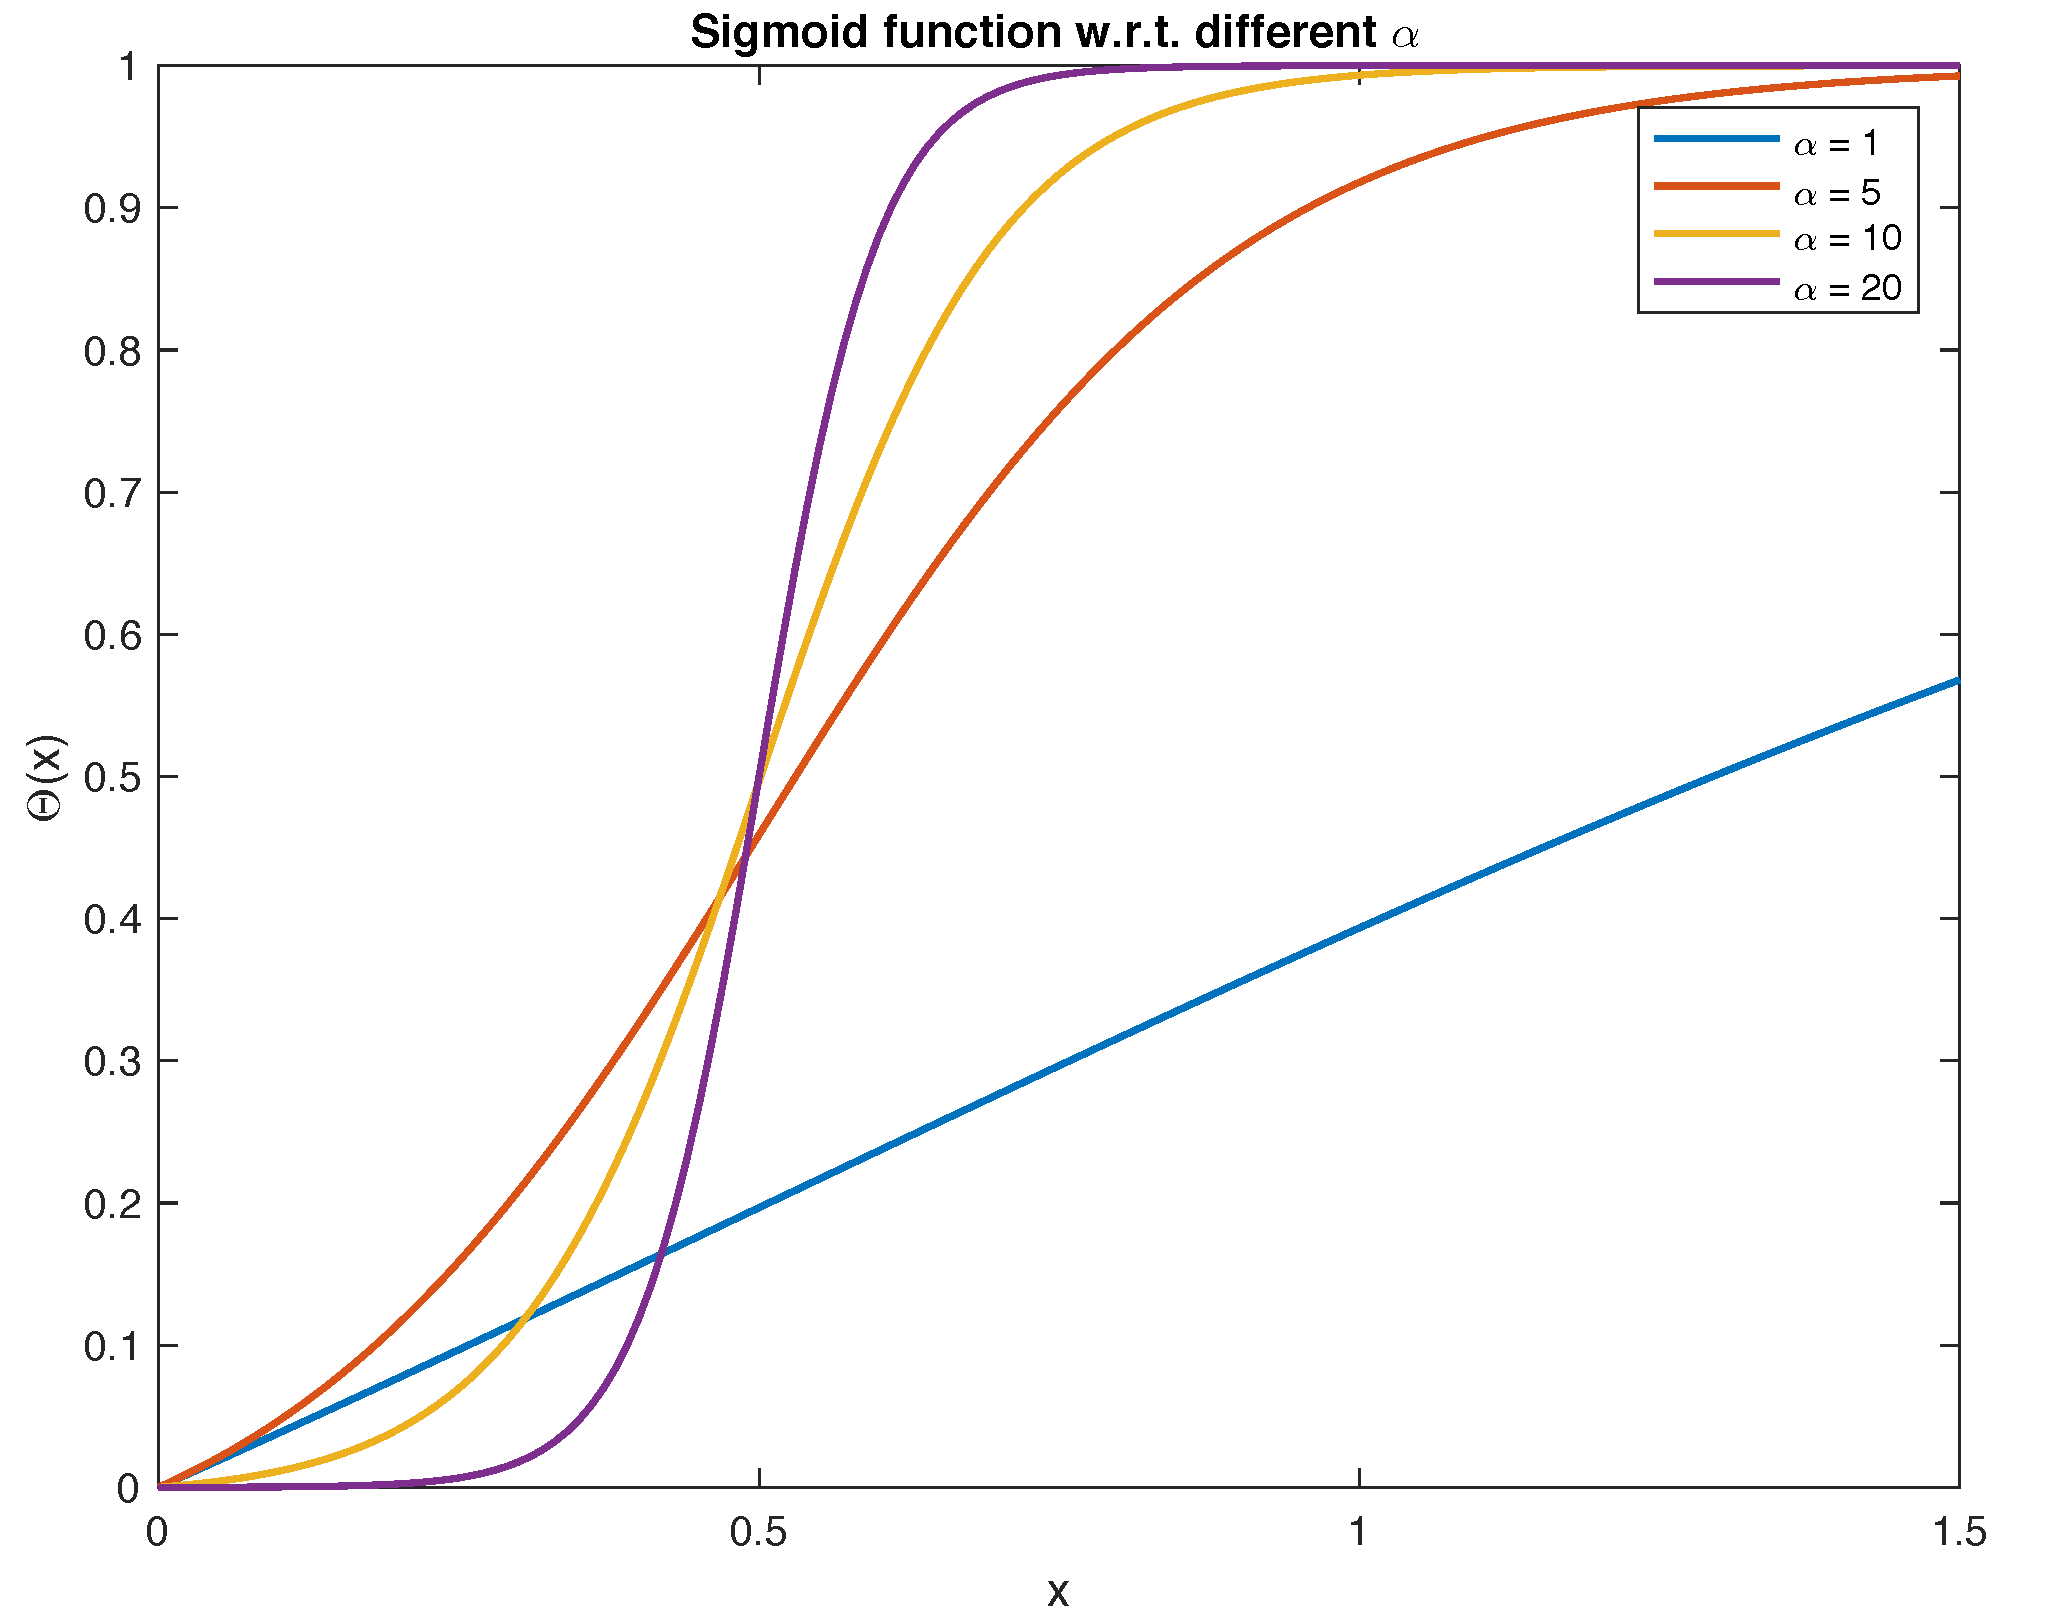
\includegraphics[height=40mm]{./figs/sigmoid_small.pdf}		
			% \caption{}
			\end{figure}
		\end{column}

		\begin{column}{0.5\textwidth}
		So sigmoid function is used to approximate 0-1 loss.
		\end{column}
	\end{columns}
	
\end{frame}

\begin{frame}
	\frametitle{Minimize number of damaged nodes (cont'd)}
	\begin{columns}
		\begin{column}{0.5\textwidth}
		\begin{figure}
			\centering
			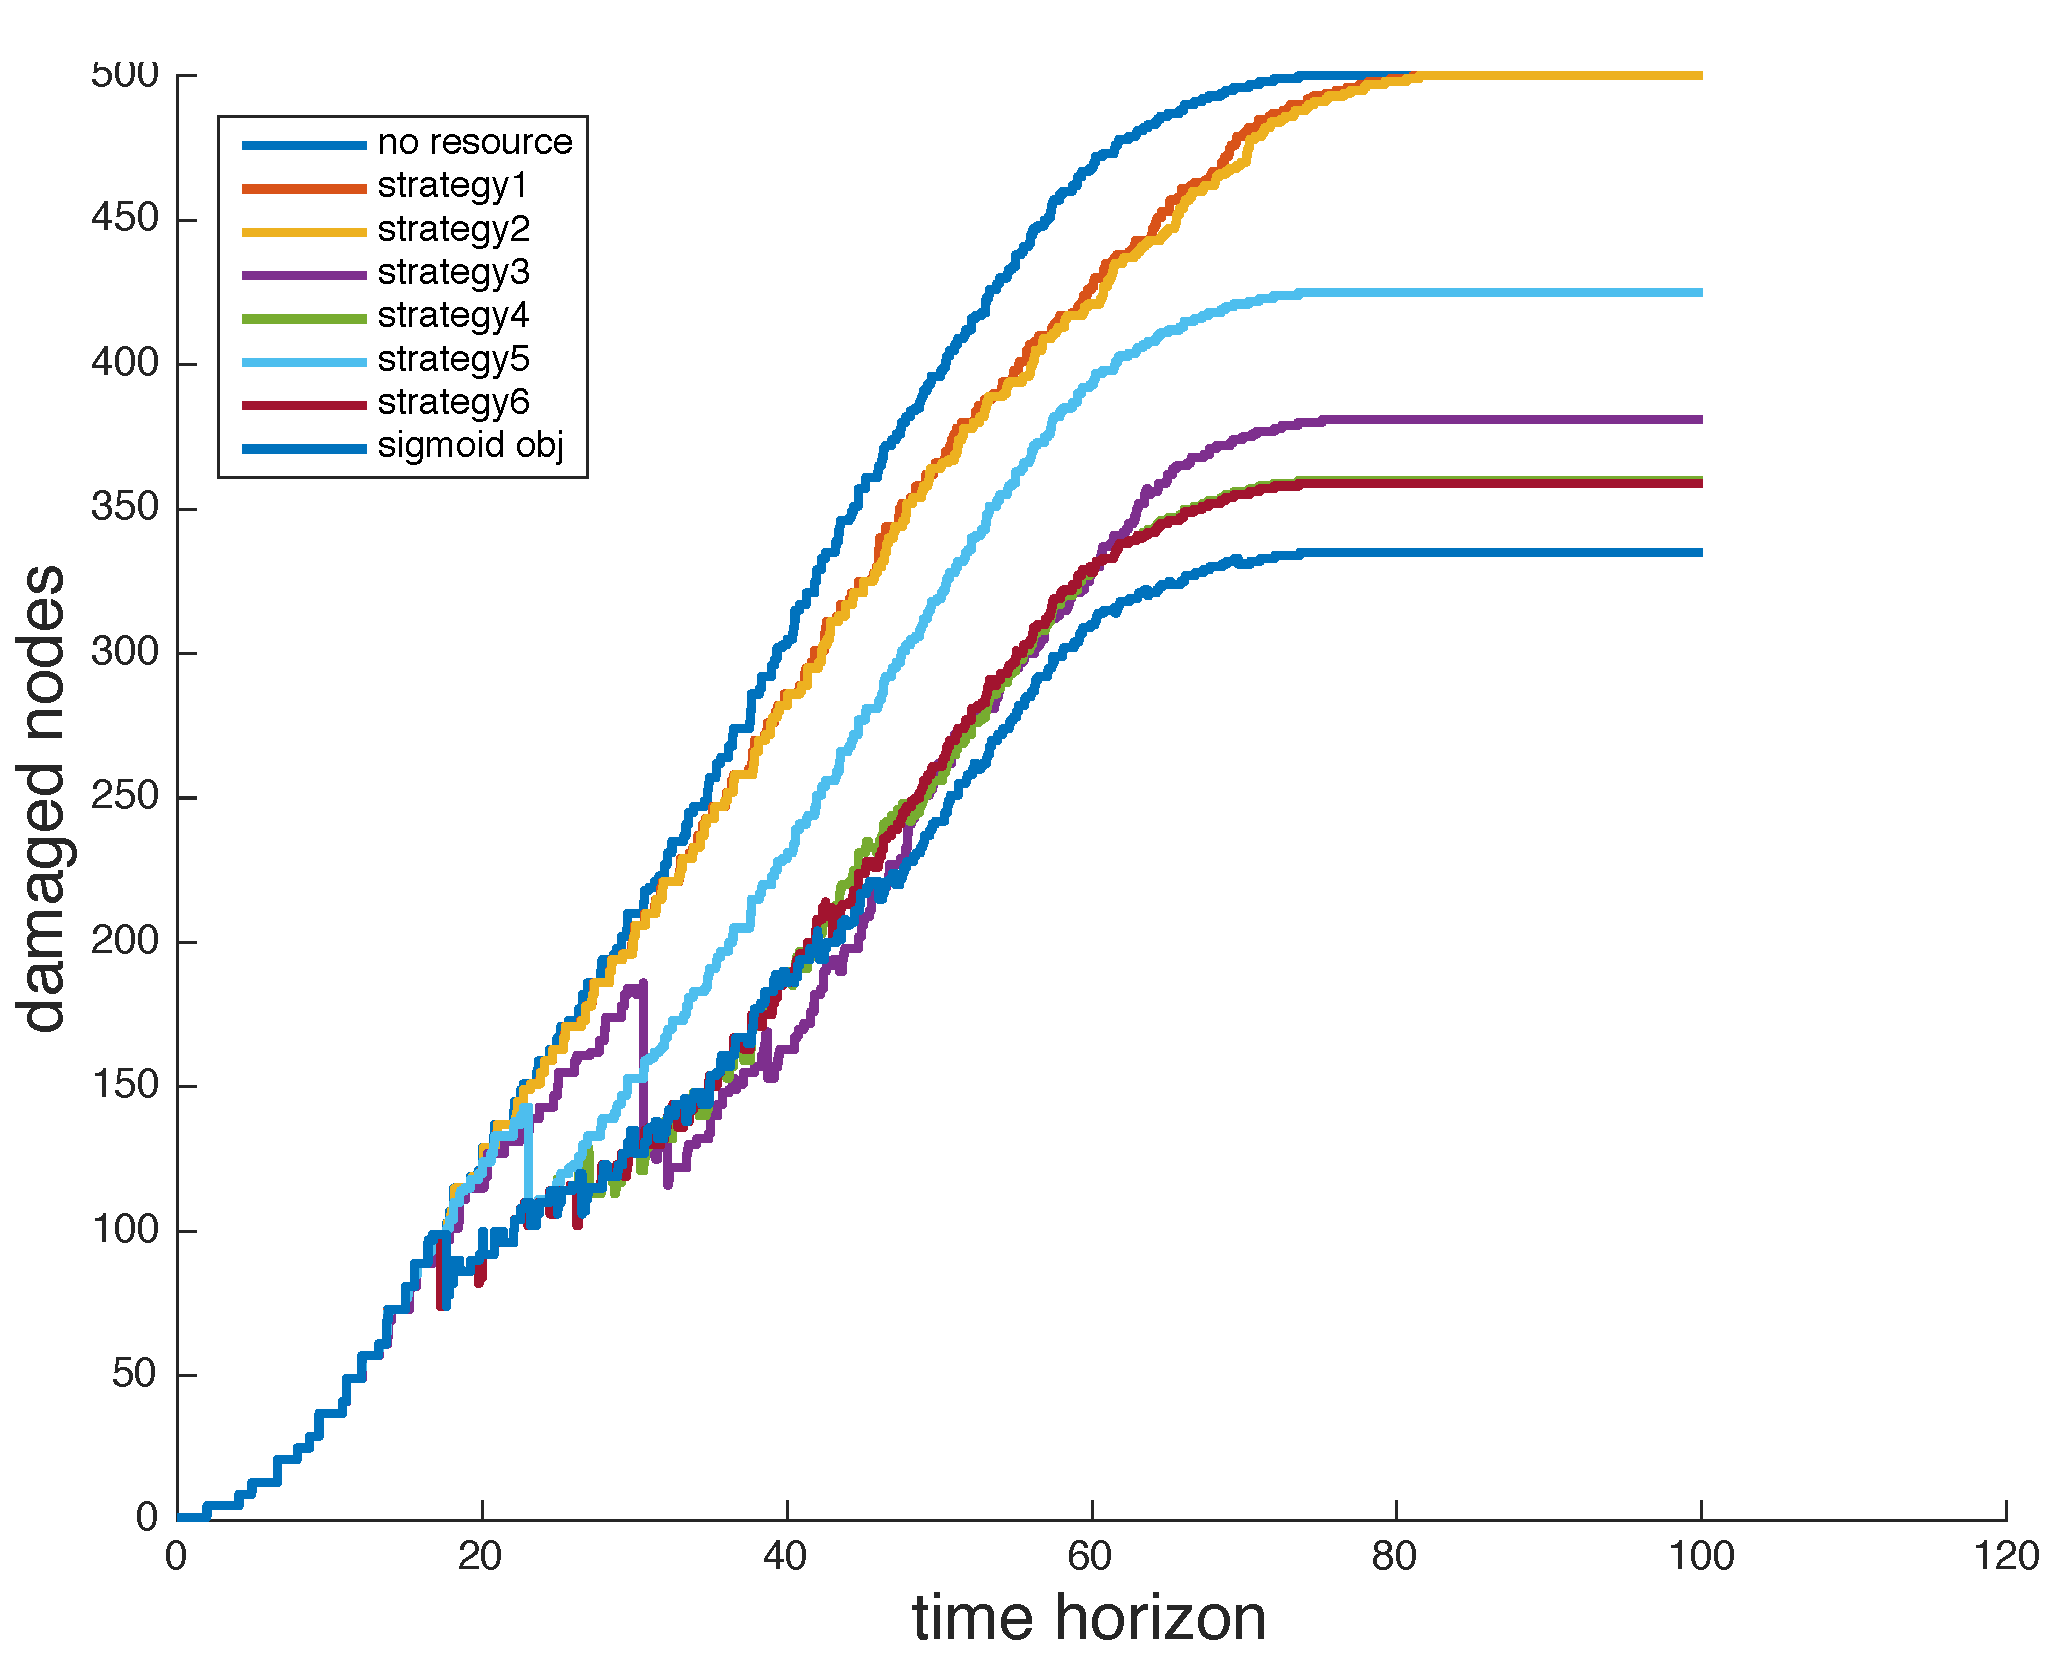
\includegraphics[height=40mm]{./figs/Grid_damaged_small.pdf}
			\caption{Damaged nodes on grid network}
			\label{fig:opt_on_grid}
		\end{figure}
		\end{column}

		\begin{column}{0.5\textwidth}
		\begin{figure}
			\centering
			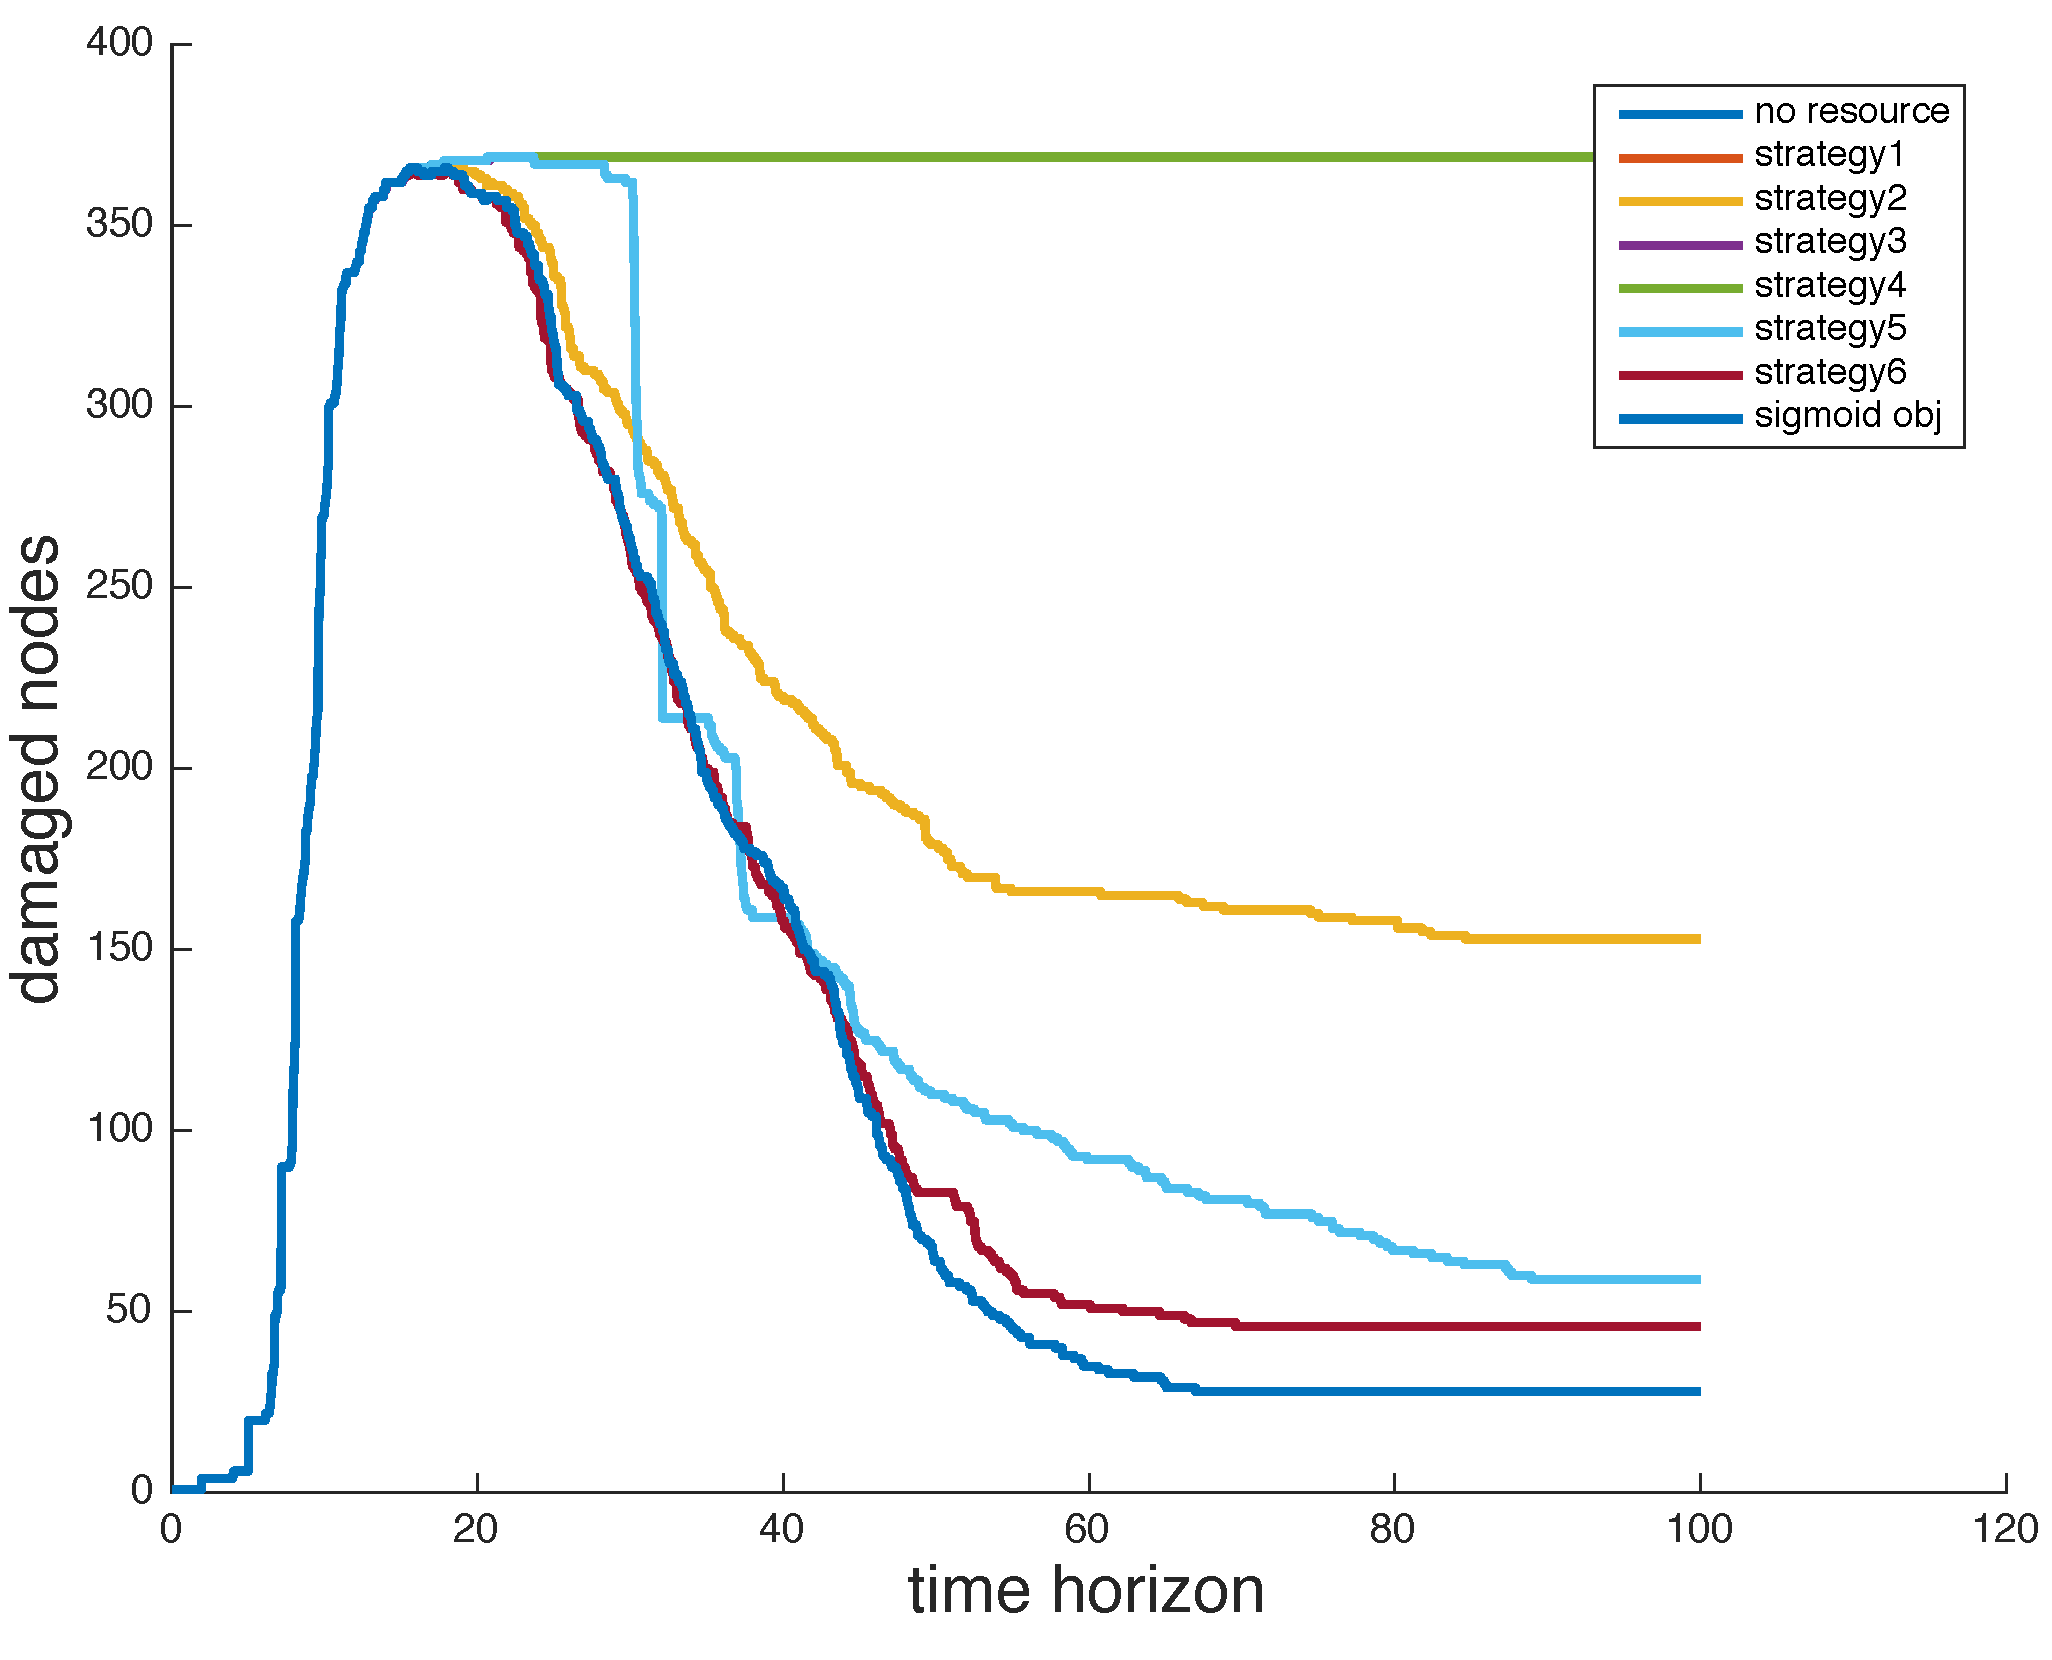
\includegraphics[height=40mm]{./figs/SF_damaged_small.pdf}
			\caption{Damaged nodes on scale-free network}
			\label{fig:opt_on_scalefree}
		\end{figure}
		\end{column}
	\end{columns}

	
\end{frame}

\begin{frame}
	\frametitle{Optimize final states}
	The objective function is simply:
	\begin{equation}
	\label{eq:obj2}
		J = \frac{1}{n} \sum_i x_T^{(i)}
	\end{equation}

	\begin{columns}
		\begin{column}{0.5\textwidth}
			\begin{figure}
				\centering
				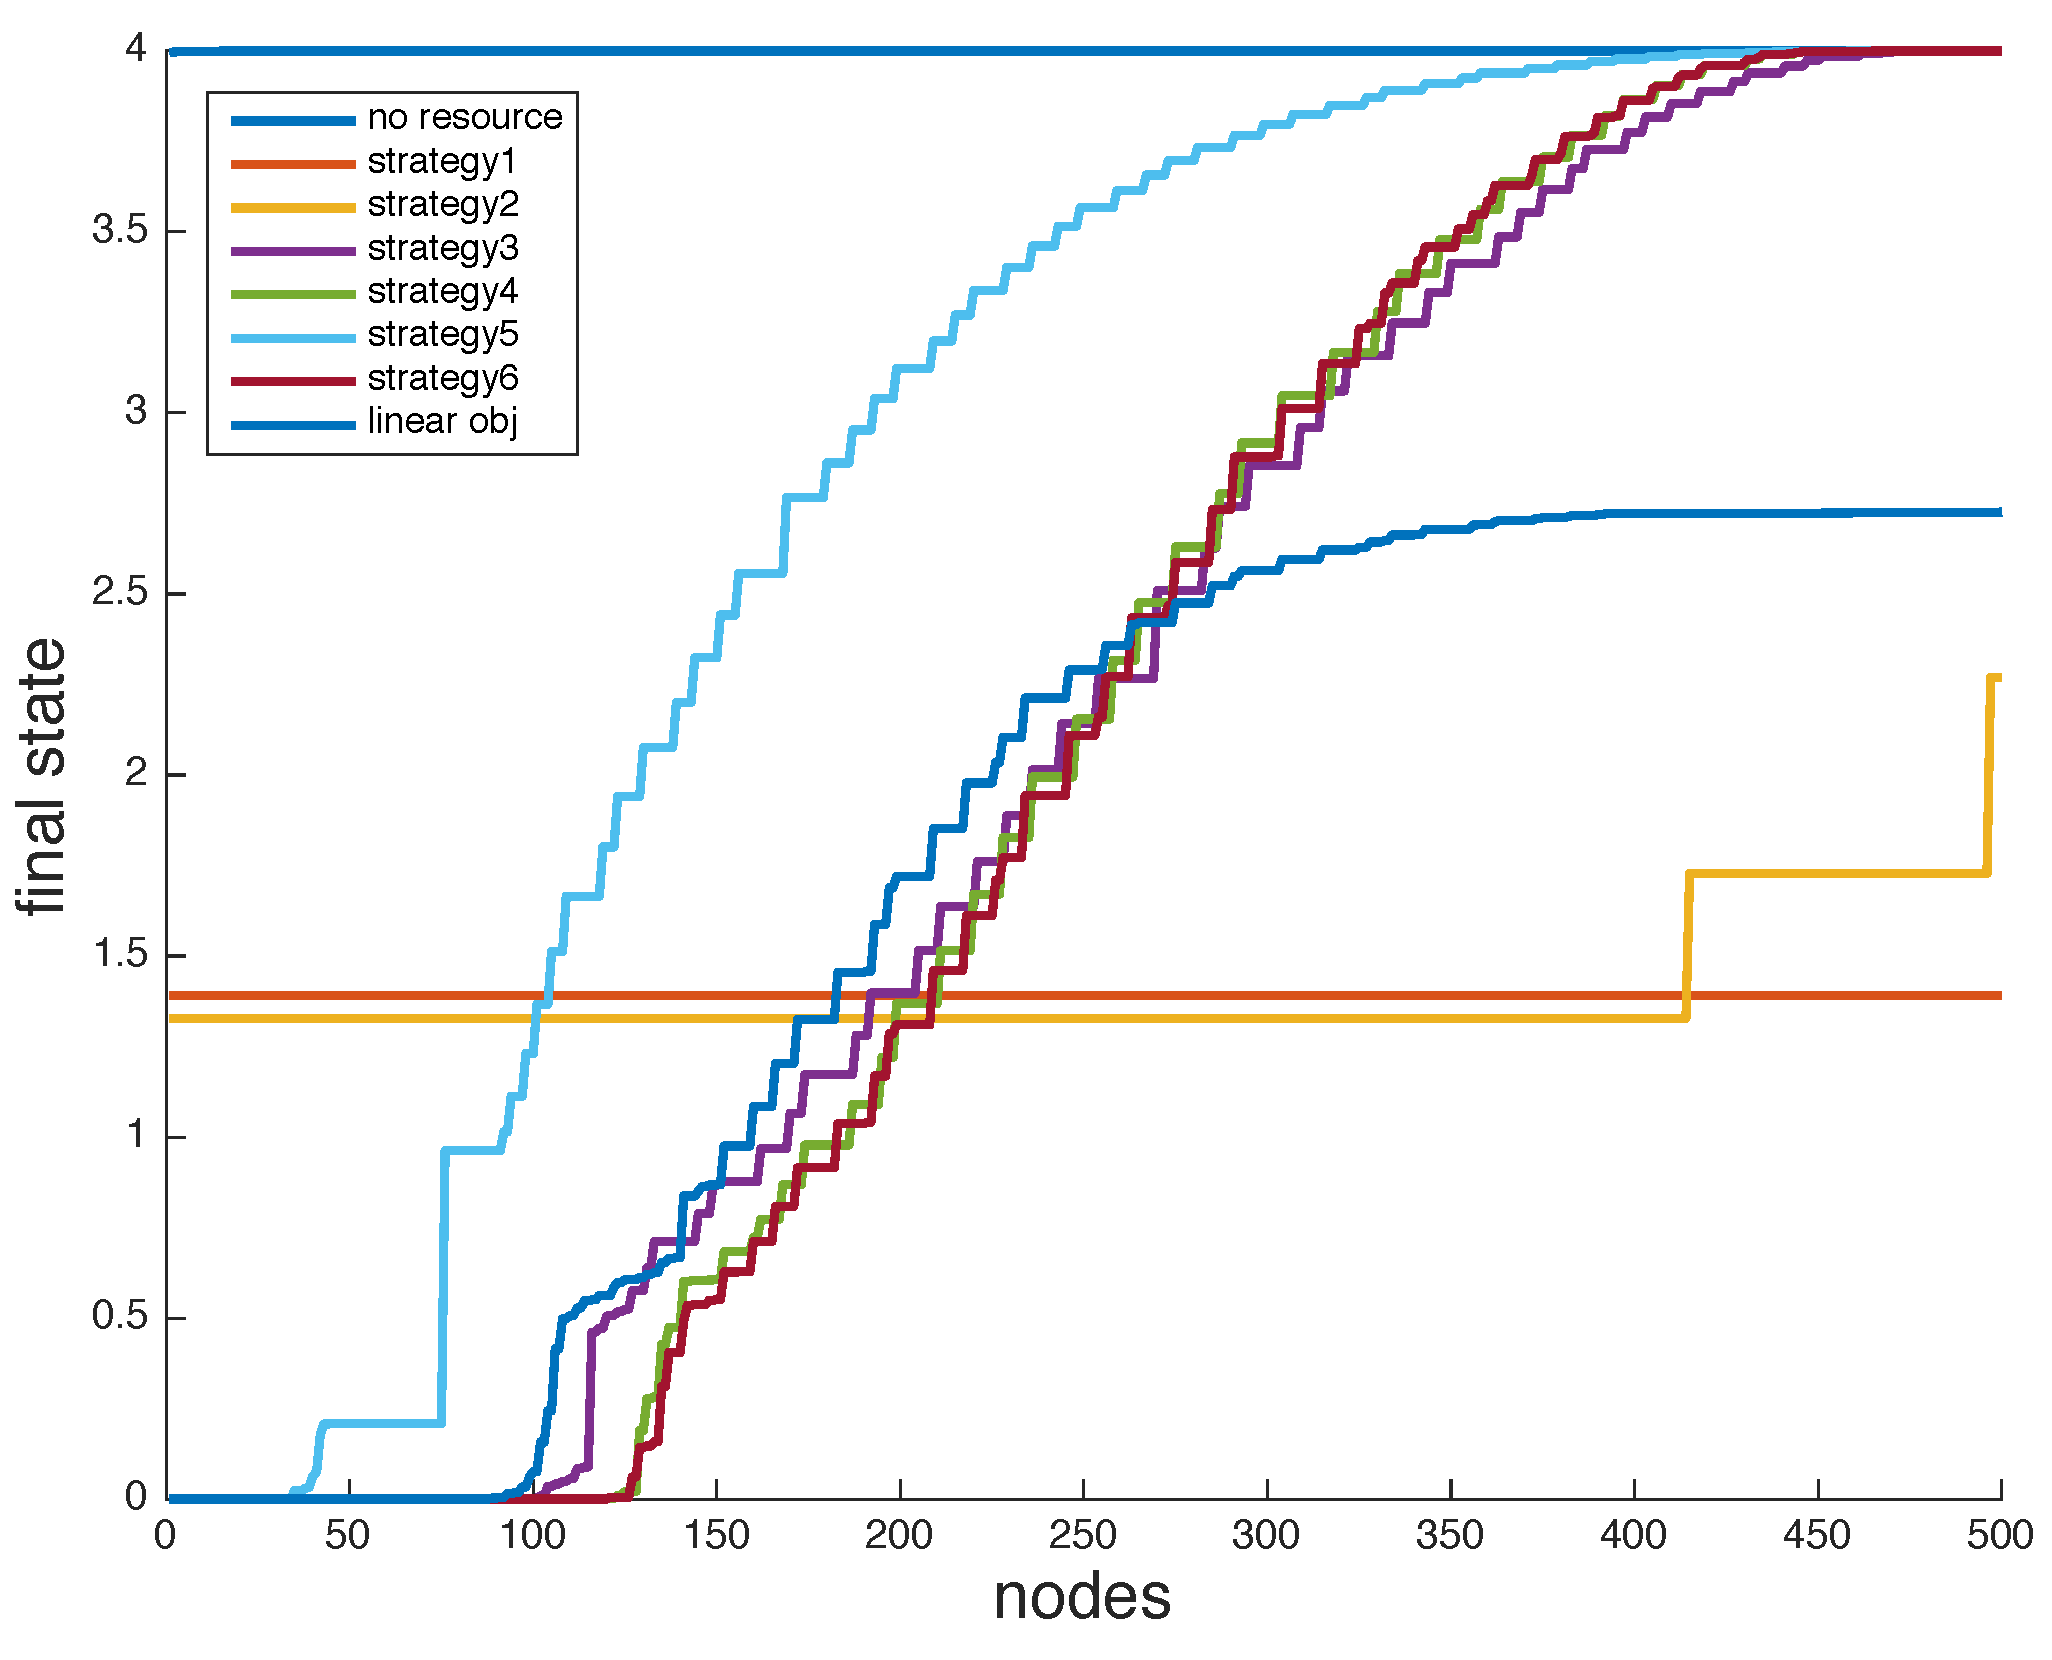
\includegraphics[height=40mm]{./figs/Grid_finalState_small.pdf}
				\vspace{-4mm}
				\caption{Final state of grid network}
			\end{figure}
		\end{column}

		\begin{column}{0.5\textwidth}
			\begin{figure}
				\centering
				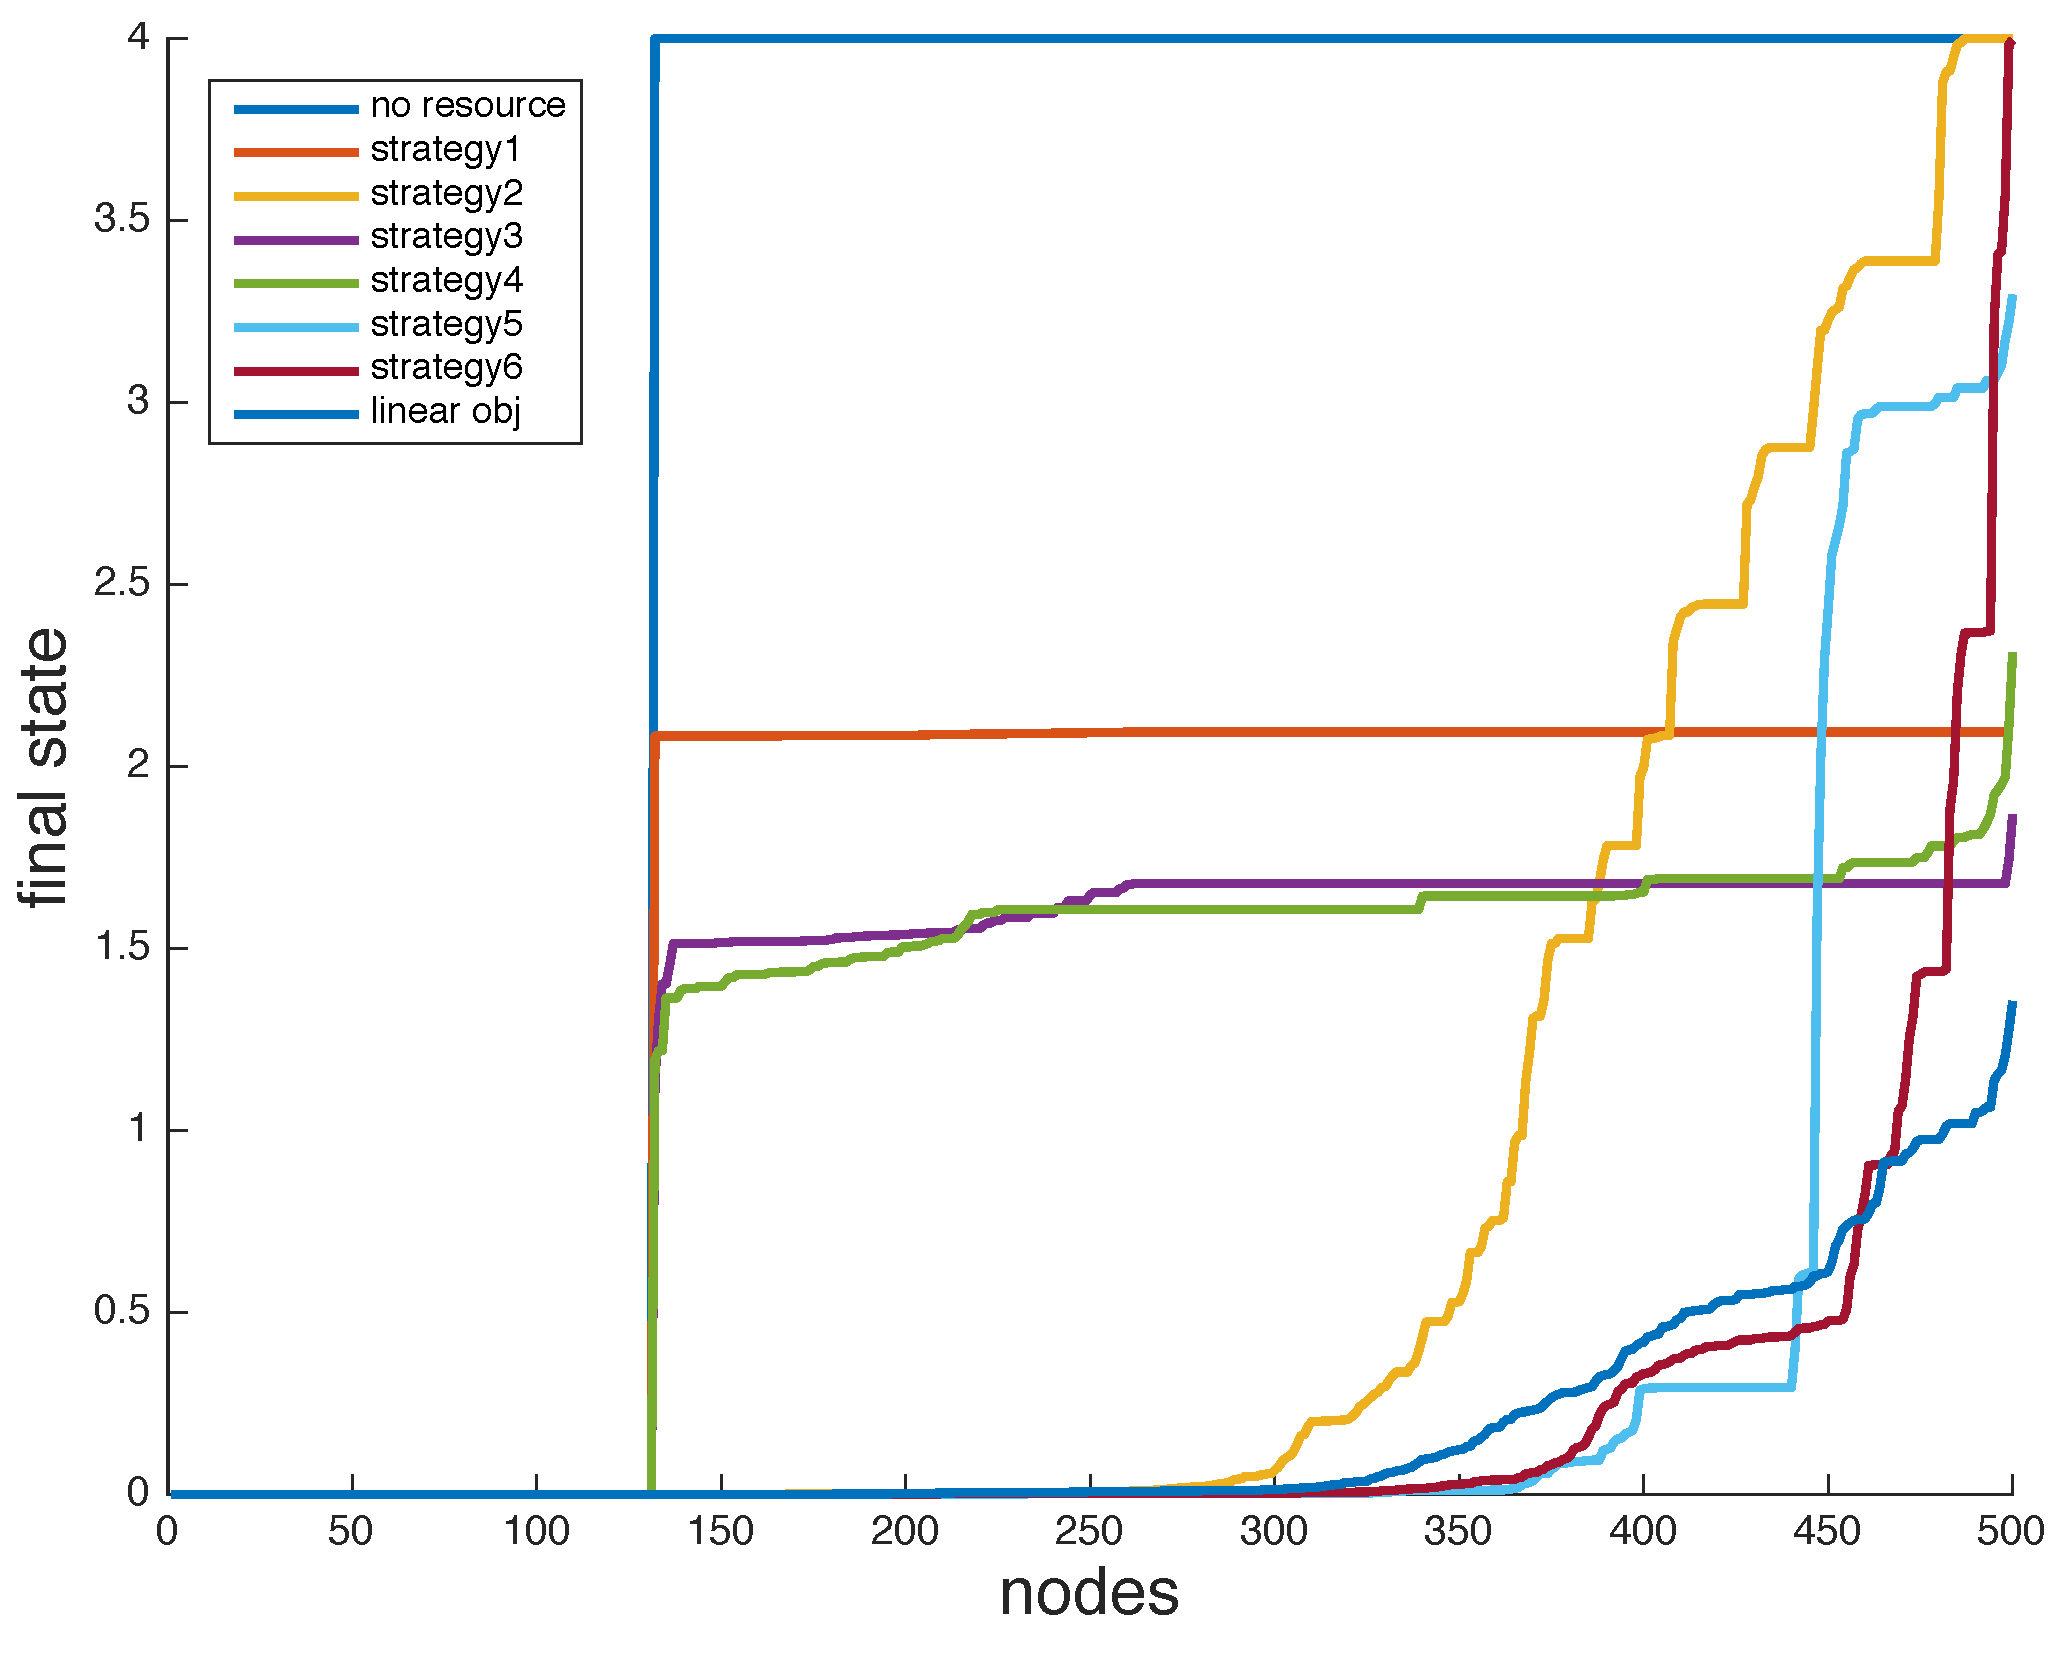
\includegraphics[height=40mm]{./figs/SF_finalState_small.pdf}
				\vspace{-4mm}
				\caption{Final state of scale-free network}
			\end{figure}
		\end{column}
	\end{columns}
	
\end{frame}


\begin{frame}
	\frametitle{Optimize Final States (cont'd)}
	
	Explanation: the horizontal line of \textbf{S1} in grid network:
	\begin{itemize}
		\item it is a stable state, which can be shown mathematically (details in our report)
		\item it can further show that \textbf{S1} is optimal w.r.t optimizing final states (details in our report)
	\end{itemize}

	\begin{columns}
		\begin{column}{0.5\textwidth}
			\centering
			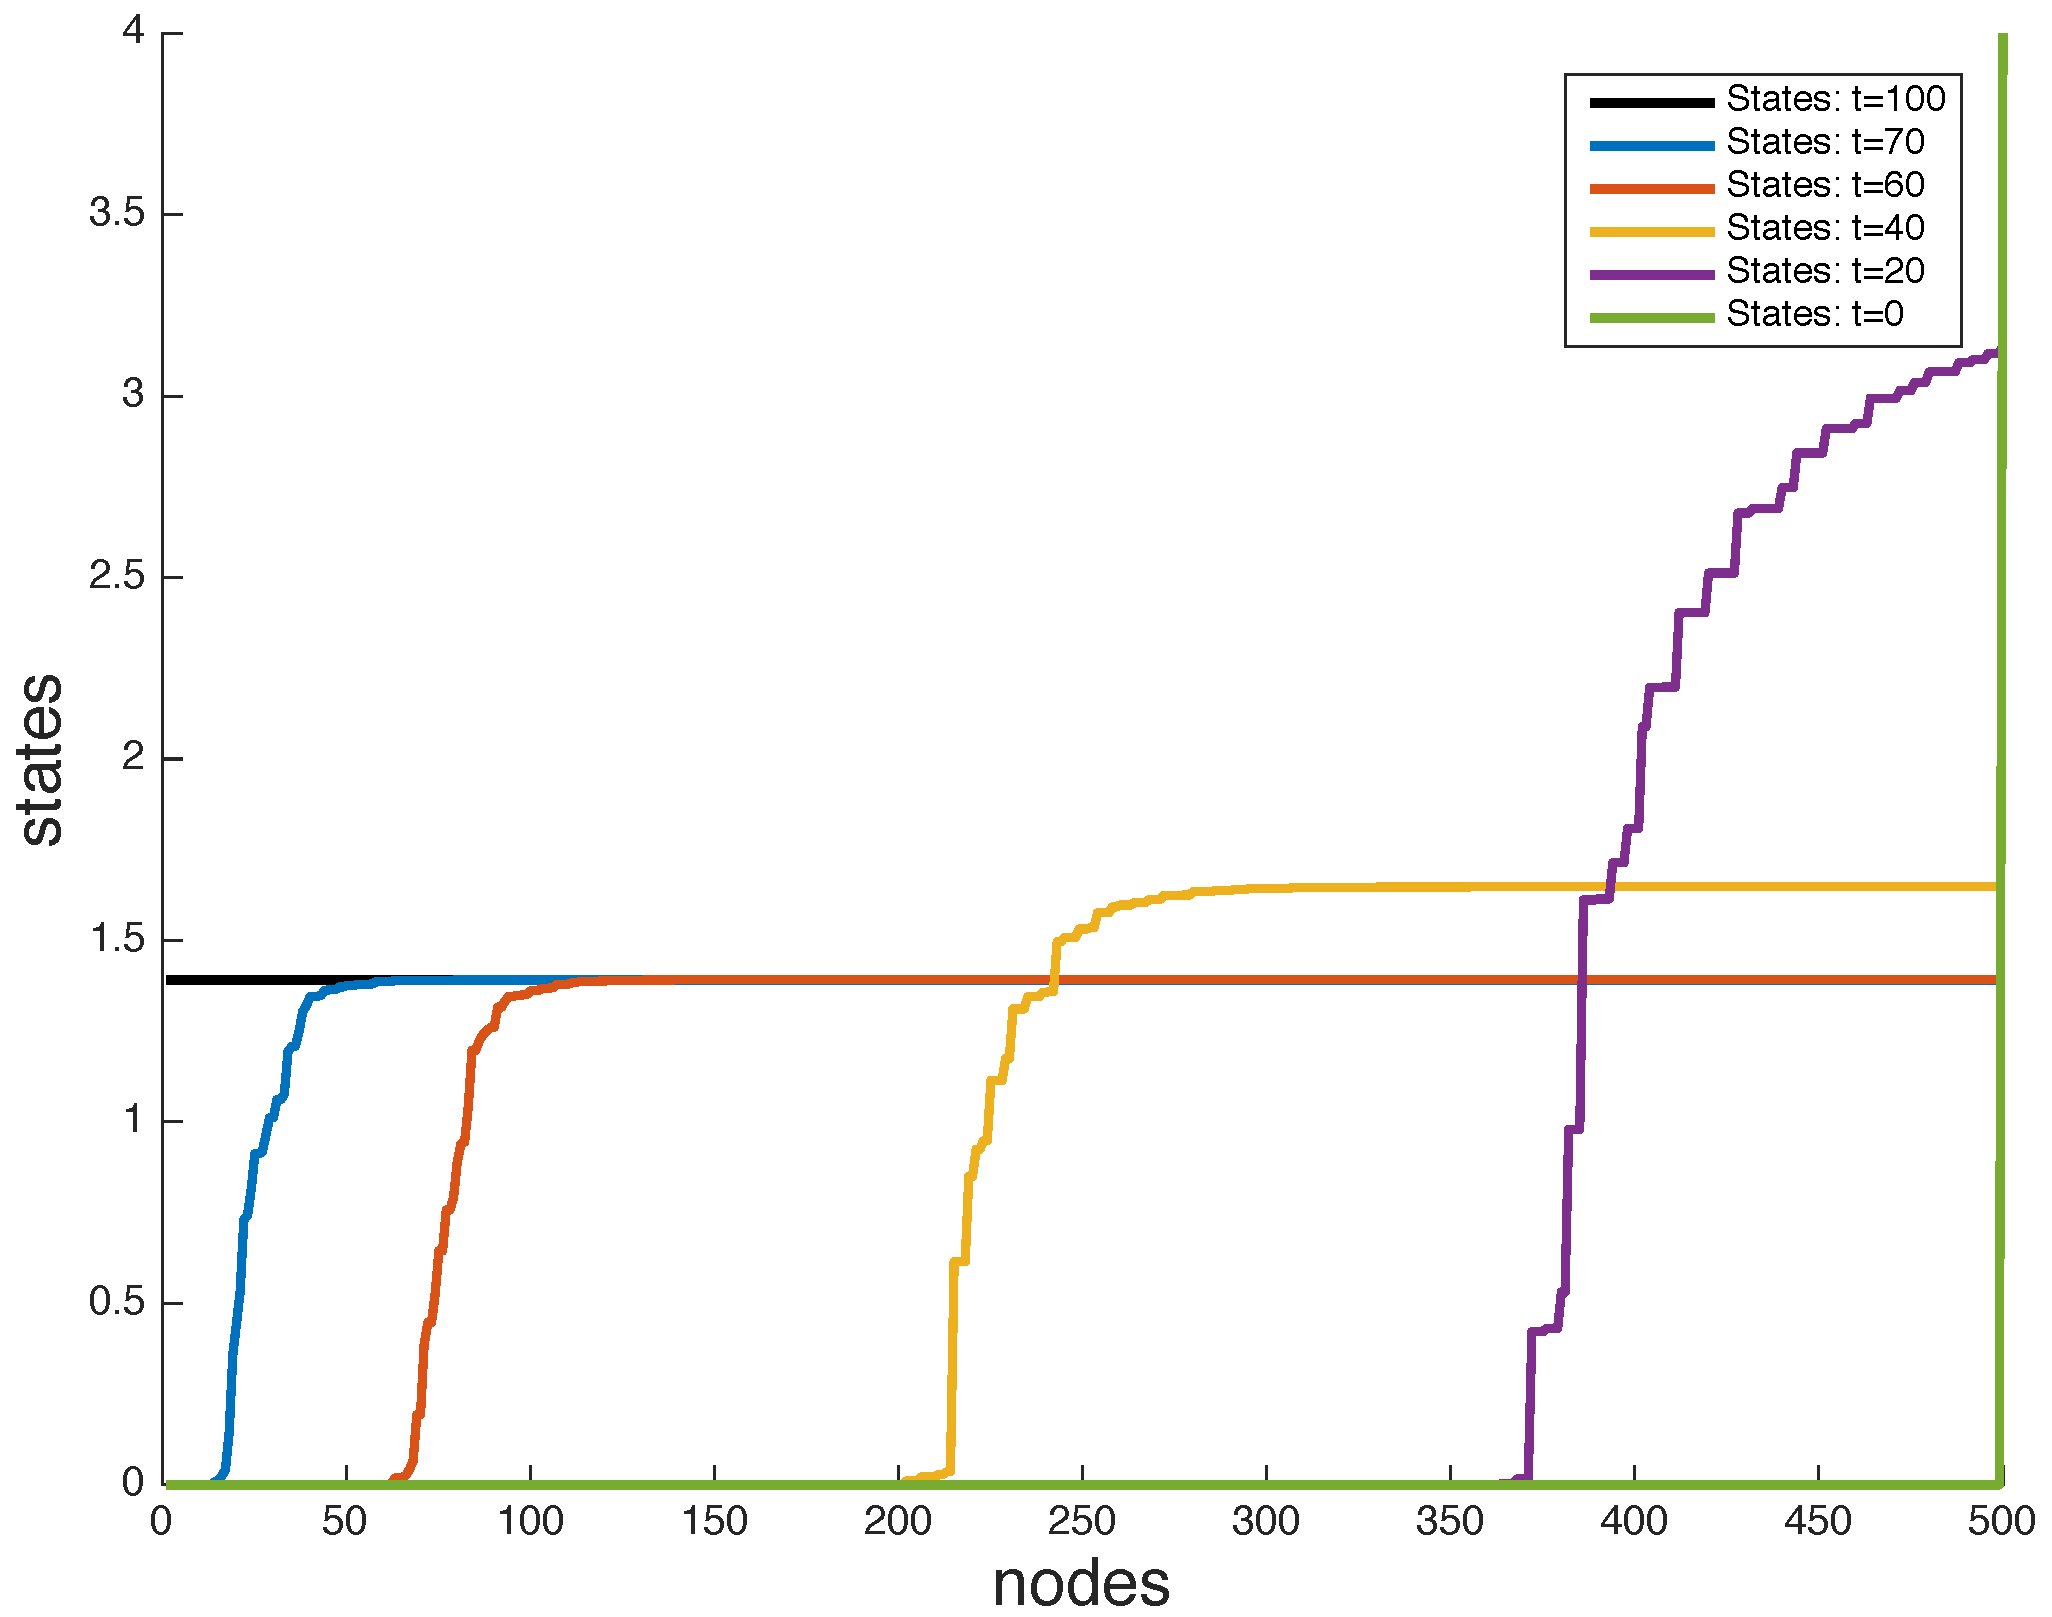
\includegraphics[height=40mm]{./figs/Grid_S1_States_small.pdf}
		\end{column}

		\begin{column}{0.5\textwidth}
			\centering
			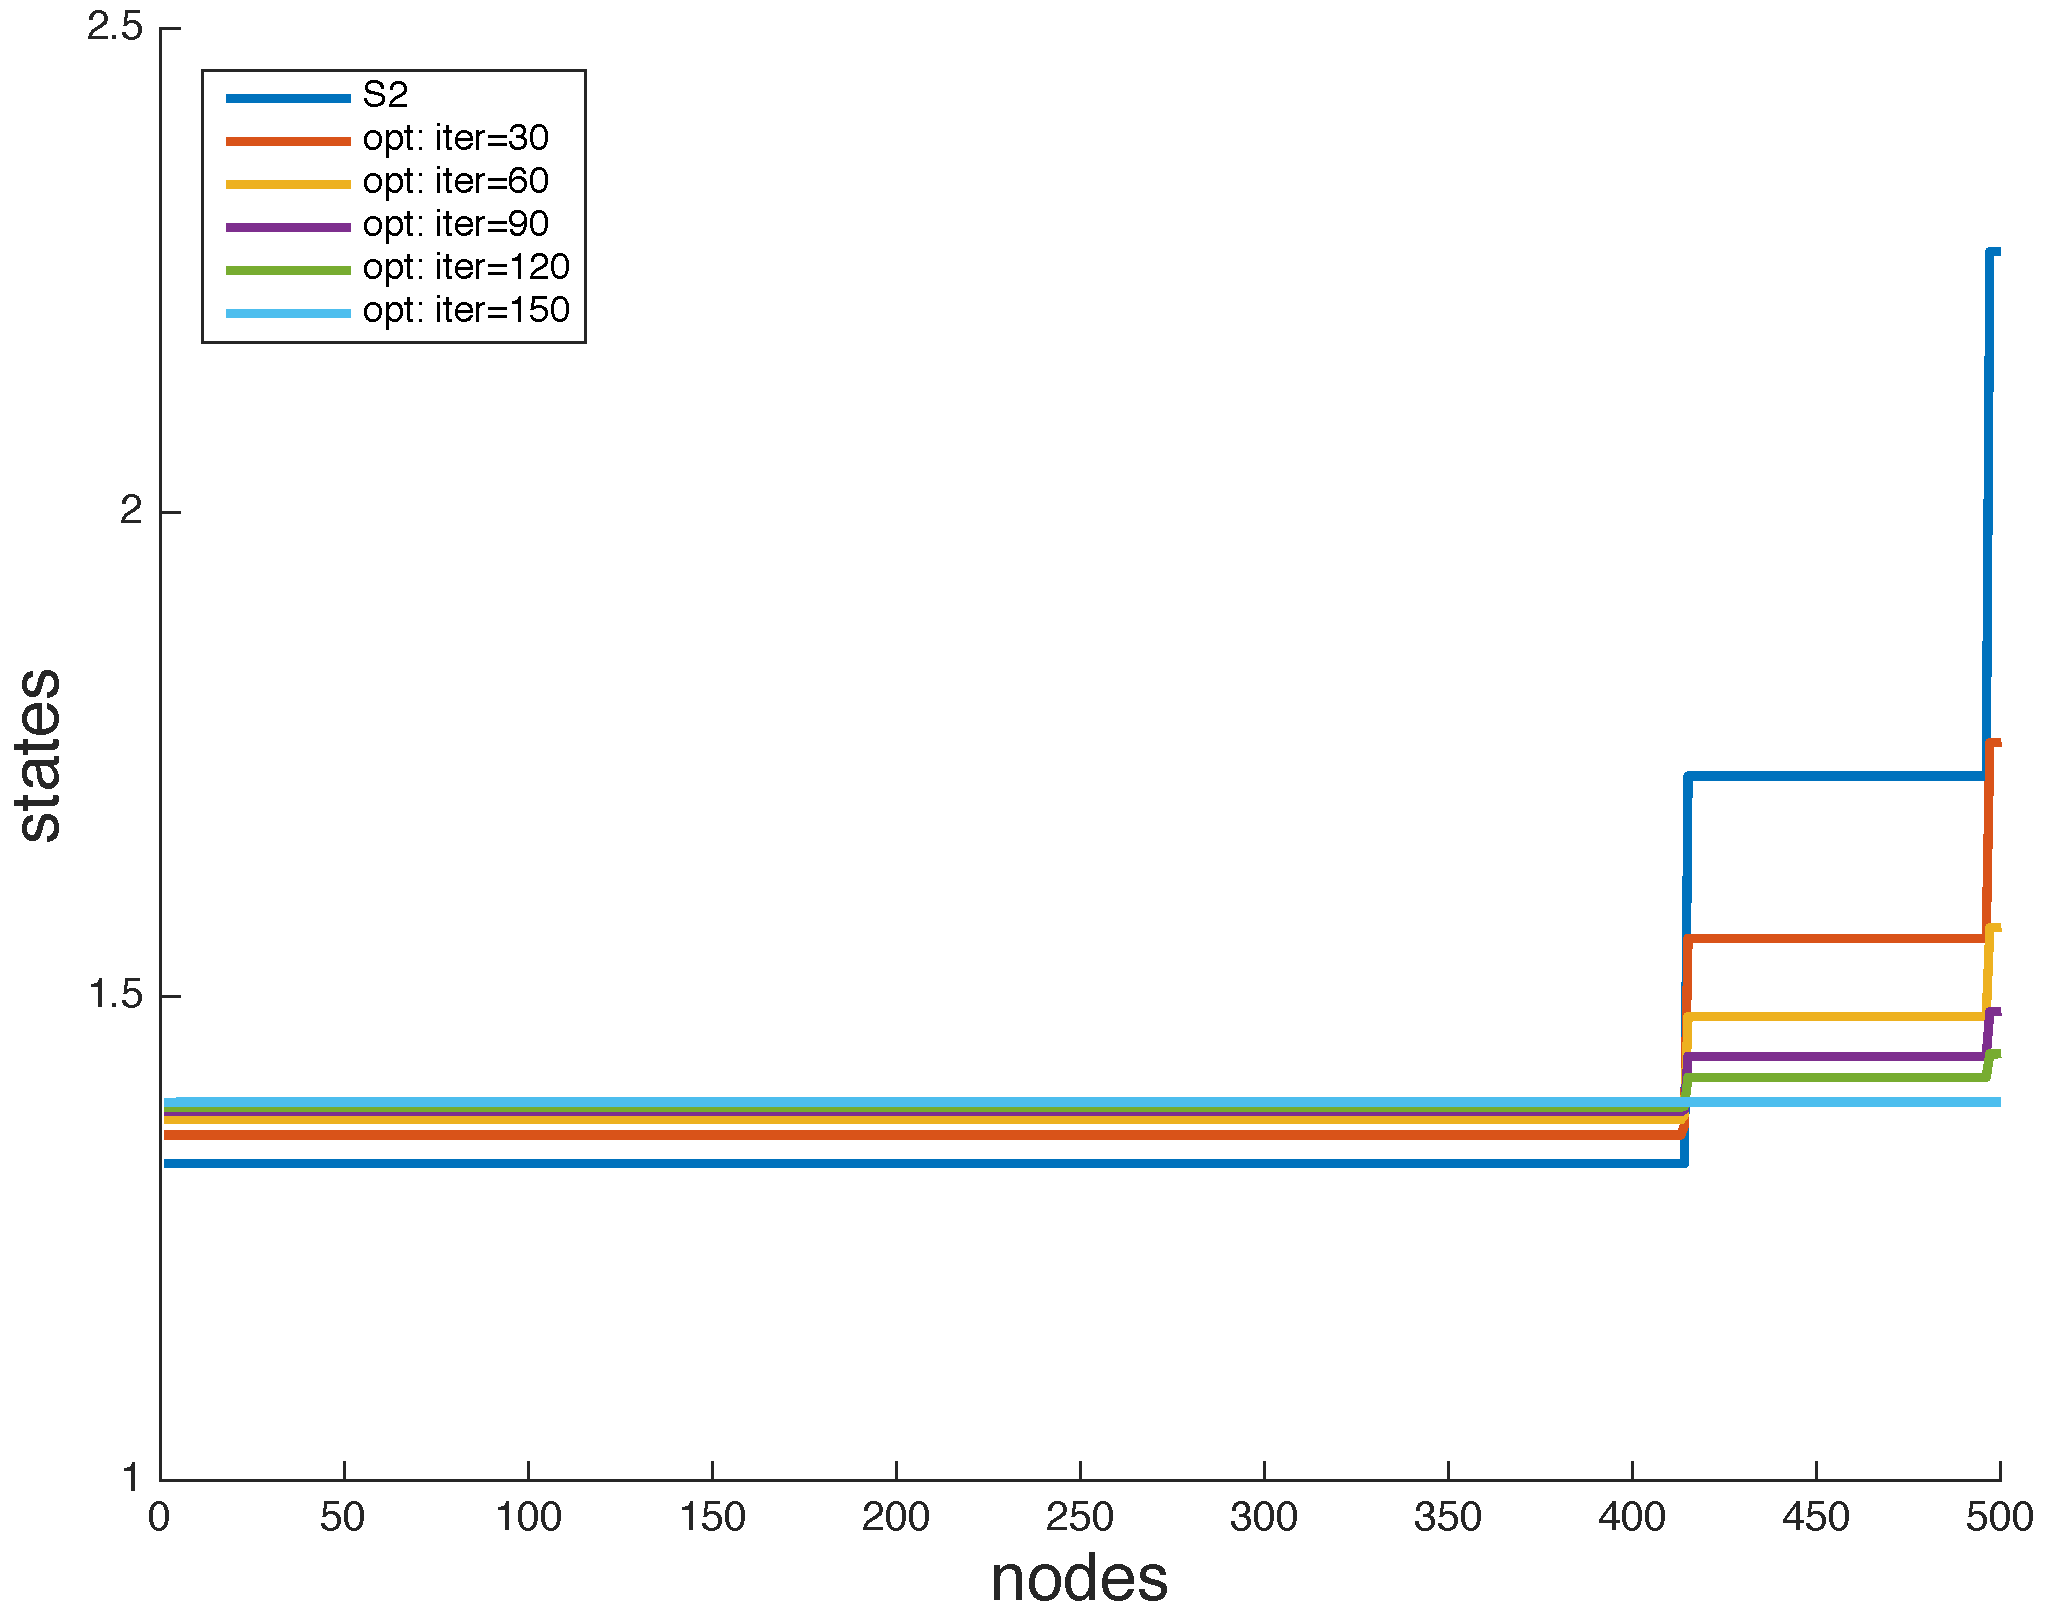
\includegraphics[height=40mm]{./figs/Grid_OptimalStates_small.pdf}
		\end{column}
	\end{columns}
	
\end{frame}

\begin{frame}
	\frametitle{Conclusion}
	We did these:
	\begin{itemize}
		\item reproduce the results of original paper\footnotemark[1]
		\footnotetext[1]{L Buzna, K Peters, H Ammoser, C K\"uhnert, D Helbing, PRE 75 (5), 056107}
		\item find the optimal strategy by solving the PDE-constrained optimization problem (however, may be a local optimum)
		\item compare the optimal strategy with these heuristic strategies on grid network and scale-free network
	\end{itemize}
\end{frame}

\begin{frame}

	\begin{center}
		\Huge Thanks for your attention!
	\end{center}
	
\end{frame}

\end{document}

